%%% This document is only for test

\documentclass{article}

%\usepackage[backend=biber]{biblatex}
%\addbibresource{dissertation.bib}

\begin{document}

This is to test a reference in bibtex. \cite{book:Shannon1997}

%\printbibliography

\bibliographystyle{unsrt}
\bibliography{dissertation}



%table template
\setlength{\arrayrulewidth}{.5mm}
\setlength{\tabcolsep}{18pt}
\renewcommand{\arraystretch}{1.2}
\begin{table}[h!]
    \centering
    \captionsetup{justification=centering}
    \caption{System specification}
    \label{table: sysspec}
    \vspace{-1em}
    \begin{tabular}{ p{20em} c }
    \hline 
    Entrance pupil diameter (EPD, mm) & 0.8\\
    Full field of view (FOV, °) & 110\\
    Effective focal length (EFL, mm) & 3.5\\
    Wavelength (nm) & 644, 546, 480\\
    \hline
    \end{tabular}
\end{table}

%template figures
\begin{figure}[h!]
    \centering
    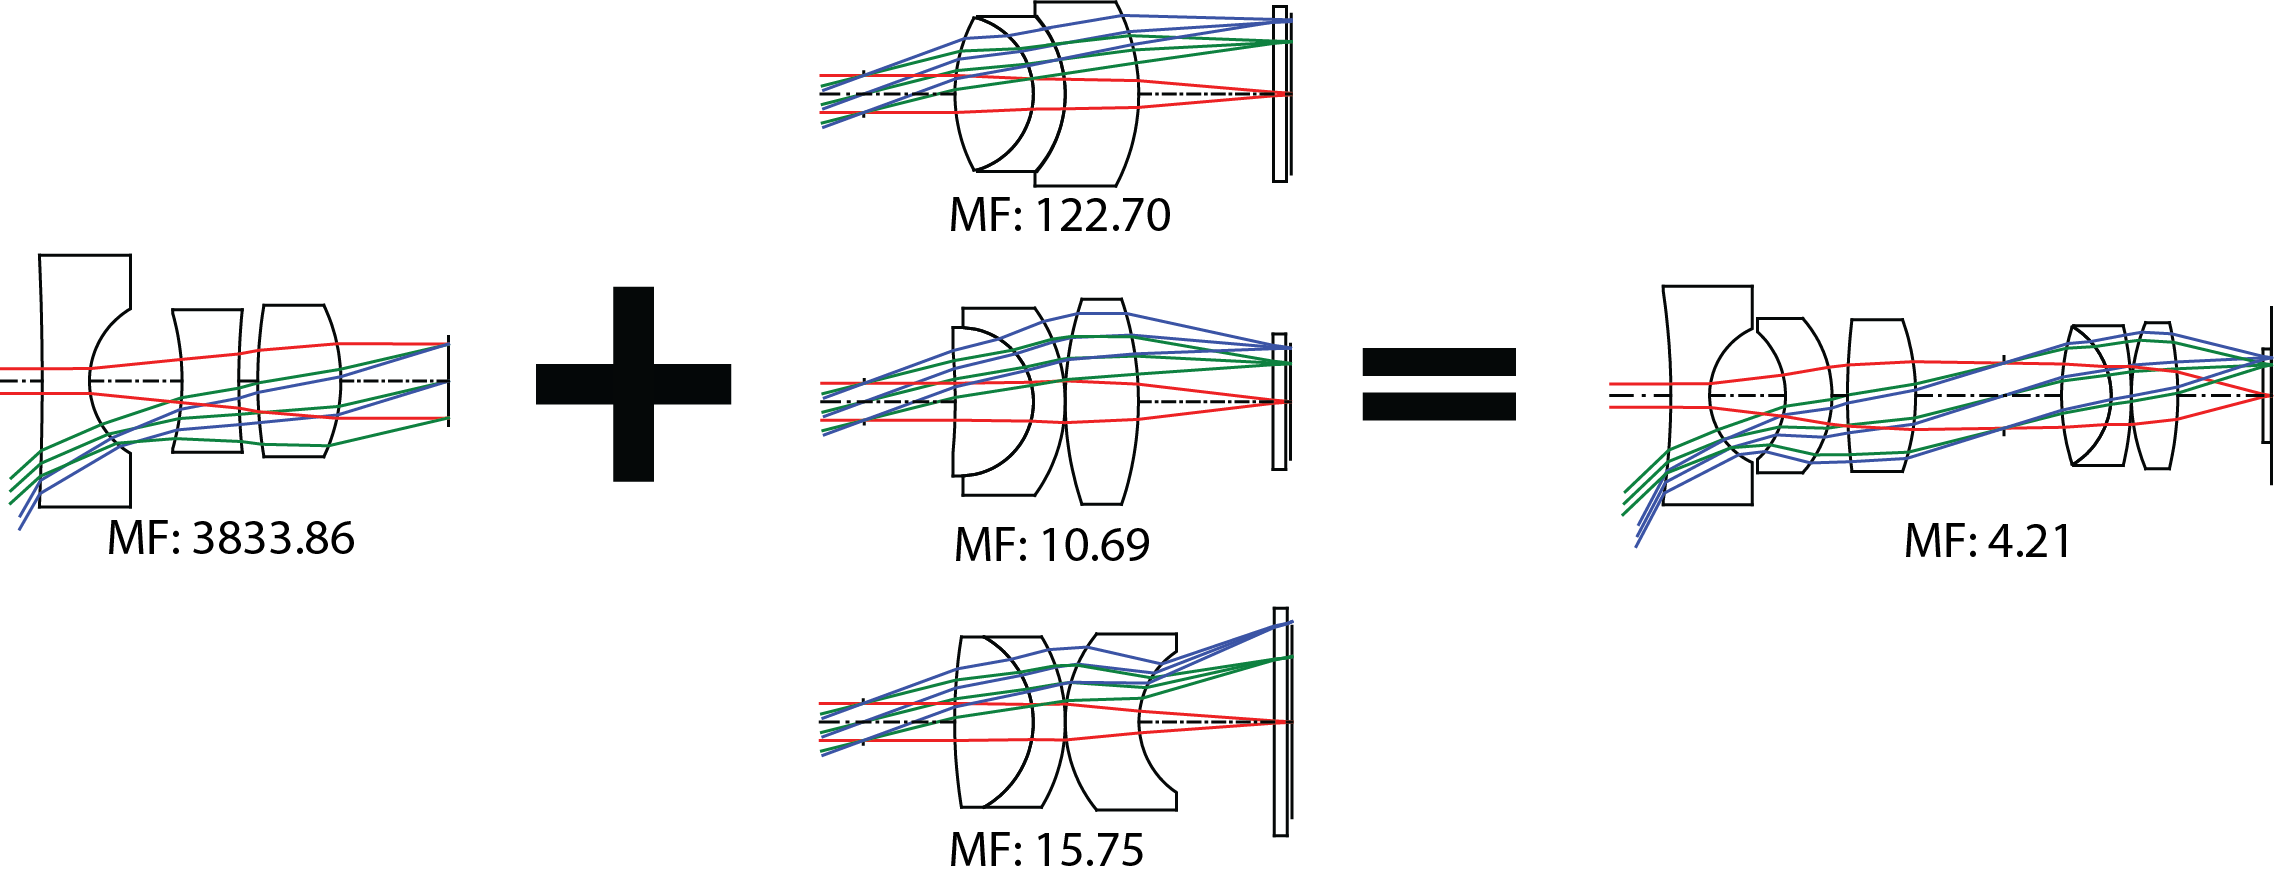
\includegraphics[width=\textwidth]{chapter-4/figures/WAL_combine.png}
    \caption{Combination of the front part and three rear parts all result in one solution.}
    \label{fig:WAL_combine}
\end{figure}
\end{document}

%template equations
\setlength{\belowdisplayshortskip}{5pt}
\setlength{\abovedisplayshortskip}{5pt}
\begin{equation} \label{eq:u1}
\hat{u}_{1} =  \left\| \overrightarrow{SA}-{\frac{\langle \overrightarrow{SA},\overrightarrow{SB}\rangle}{\langle \overrightarrow{SB},\overrightarrow{SB}\rangle}}\overrightarrow{SB} \right\| 
\end{equation}
\setlength{\belowdisplayshortskip}{10pt}
\begin{equation} \label{eq:u2}
\hat{u}_{2} = \left\| \overrightarrow{SB} \right\|
\end{equation}
%template 2 - split one line into two
\setlength{\belowdisplayshortskip}{5pt}
\setlength{\abovedisplayshortskip}{5pt}
\begin{equation} \label{eq: MFminCon}
\begin{split}
& \text{minimize}\;\; MF(\textbf{x}) \\
& \text{subject to}\;\; g(\textbf{x}) = 0
\end{split}
\end{equation}
%template subequations
\setlength{\belowdisplayshortskip}{5pt}
\setlength{\abovedisplayshortskip}{5pt}
\begin{subequations} 
\begin{align}
& \nabla_\textbf{x}\mathcal{L}(\textbf{x},\lambda)=\nabla_\textbf{x}MF(\textbf{x})-\lambda\nabla_\textbf{x}g(\textbf{x})=0 \label{eq: LagCondition1} \\
& \nabla_\lambda\mathcal{L}(\textbf{x},\lambda)=g(\textbf{x})=0 \label{eq:LagCondition2}
\end{align}
\end{subequations}